\documentclass[main.tex]{subfiles}
\begin{document}

\onlyinsubfile{
\pretitle{}
\posttitle{}

% Title page content
\title{\LARGE \textbf{ARIO: the Adaptive Regional Input Output model} \\[0.5cm]
  \huge An extensive indirect impact assessment model and its python implementation.}
\author{}
\date{\large \today}

\maketitle
}

\notinsubfile{\chapter{Description of the ARIO indirect economic cost model}\label{ch_boario}}

\onlyinsubfile{
\section{Introduction}
\label{sec:intro-model}

The Adaptive Regional Input Output or ARIO model is an indirect economic impact
assessment model originally presented in
\textcite{hallegatte-2008-adapt-region, hallegatte-2013-model-role}. The ARIO
model extends the ``traditional'' input-output (IO) framework commonly used for
indirect impact assessment with additional adaptive dynamics, and has been
widely used in the literature. Many different implementation exist sometime
assuming different modeling choices. This document attempts at producing an
up-to-date description of the model corresponding to its python open-source
implementation \texttt{boario} (\url{https://spjuhel.github.io/BoARIO/}), and
serves as a formal reference for the studies using the package.
}

\section{Short Description}
\label{sec:depth-descr-ario}

This section briefly presents the ARIO model. We strongly encourage the reader to consult the full
description~\Cref{sec:full-description-ARIO} where we provide a more
in depth analysis of the different components of the model, as well as a
reflection on the parameters values that were used in the literature.

\subsection{Model structure}
\label{sec:model_struc}

Our basis for the structure of the model is very similar to the one described
in~\textcite{hallegatte-2013-model-role} with some additions
from~\textcite{guan-2020-global-suppl}. We model the economy as a set of economic \emph{sectors}
and a set of \emph{regions}. These regions and sectors are entirely defined by
the \acrfull{MRIOT} used, thus the model itself is agnostic from any specific
typology of regions and sectors. We use the term \emph{industry} to designate a
specific couple of a sector and a region, i.e., our basic productive agents.
Each industry produces a unique product which is assumed to be the same for all
industries of the same sector. Each industry keeps an inventory of inputs it
requires for production. These inventories are expressed for each
input as the number of simulation steps\footnote{Usually one day, but this is
  actually a modeling choice in BoARIO.} an industry can produce with said input
while maintaining its current production level. Each industry answers a total demand consisting of a
share of the final demand (accounting for household consumption, public spending
and private investments) of all regions (i.e., both local demand and export) and
a share of the intermediate demand (made up of inputs inventory resupply
requirement from all industries). An initial equilibrium state for the economy is built based on
the MRIOT. The model then describes how a local
shock (or multiple ones)--either in production, demand or both--affects the
dynamics of each industry for a chosen number of steps. The model can be
described as four modules: \emph{production}, \emph{distribution and inventory},
\emph{orders}, and \emph{overproduction}, which we present in the
\Cref{sec:full-description-ARIO}. \Cref{fig:boario_sketch_1} gives an overview
of the process of advancing the model by one step.

\begin{figure}[h]
  \centering
  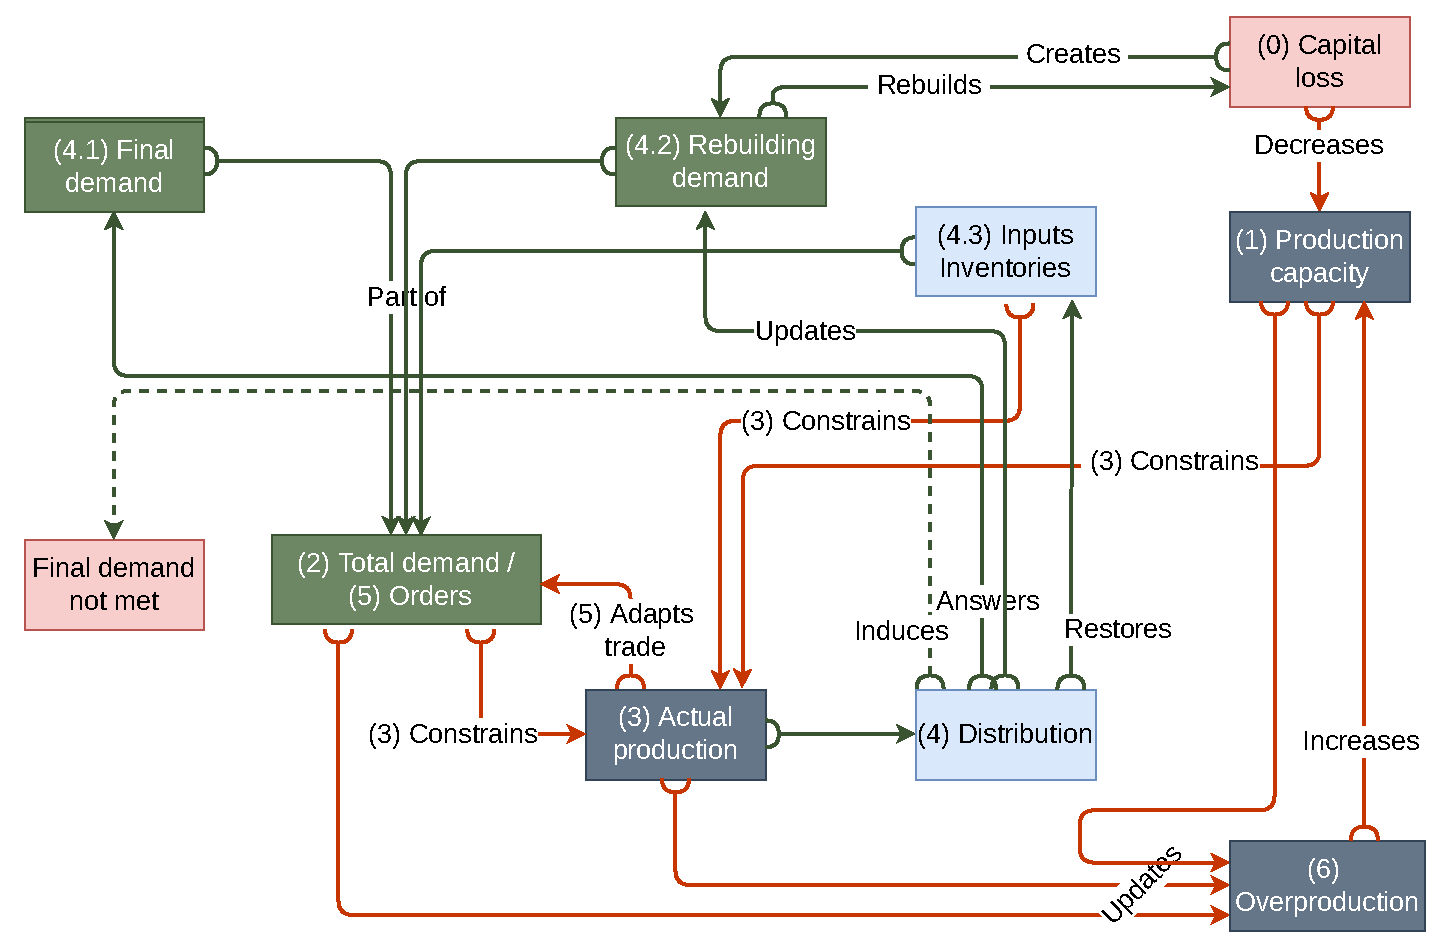
\includegraphics[width=0.70\textwidth]{imgs/BoARIO-diagram-10.pdf}
  \caption[BoARIO process diagram]{\small Diagram of one step in BoARIO
    from the point of view of a specific sector. We use productive capital
    losses as a shock in this case. If the sector has suffered capital
    losses (0), its production capacity decreases accordingly (1). Total demand
    addressed toward the sector is computed (2). Based on production capacity,
    total demand and current input inventories, actual production is computed
    (3) and required inputs are deducted from inventories. Sector's production
    is proportionally allocated towards final demand (4.1), rebuilding demand
    (4.2) and input
    inventories resupply (4.3). Final demand that could not be met
    is registered as a loss. The rebuilding production received by the sector
    is deducted from capital losses. The sector makes and adapts its
    resupplying orders based on its current inventories and the production level
    of its suppliers (5). Last, depending on total demand, production capacity
    and actual production, the sector updates its overproduction factor (6).}
  \label{fig:boario_sketch_1}
\end{figure}


\subsection{Qualitative behavior}
\label{sec:qualitative-behavior}

In order to present a general overview of the dynamics of the ARIO model,
we define the concept of \emph{shortage} in the context of the ARIO model, and
outline four elementary responses an industry may exhibit following a shock in~\Cref{fig:ario-responses}.

\awesomebox{0pt}{\faCogs}{black}{
  \textbf{Shortage}: We say that a \emph{shortage} happens, when at least one
  industry reduces its production output because it considers that at least one
  of its input is too scarce (See \Cref{sec:invent-constr} for a more formal
  definition).
}

As such shortages are a very important aspect of the ARIO model. Indeed, as
observed in later chapters, as long as no shortage happens, the model behaves
mostly linearly (indirect costs remain linear relative to the direct costs). Conversely,
when a shortage occurs during a simulation (and is significant, \emph{i.e.},
lasts for more than a few steps), the relationship between indirect and direct
losses shifts to a non-linear one, even more so when the initial shortage
cascades into subsequent ones. This non-linearity can already be explained intuitively:
as a shortage happens it acts as a new shock to the model, and as such a new
source of loss. Longer and more pronounced shortages are also more prone to cascade
into other shortages, acting as multipliers of the initial shock, thus leading
to the non-linearity.

The way an industry responds following a shock depends on the presence of a
rebuilding demand and the values of parameters. The responses showed
in~\Cref{fig:ario-responses} do not fully capture the complexity emerging from
actual simulations, but are a good basis to understand how the model behaves. We
differentiate the ``rebuilding'' and ``recovery'' cases depending on whether the
model has to answer a reconstruction demand to recover from the disaster or not.

\begin{figure*}[ht]
  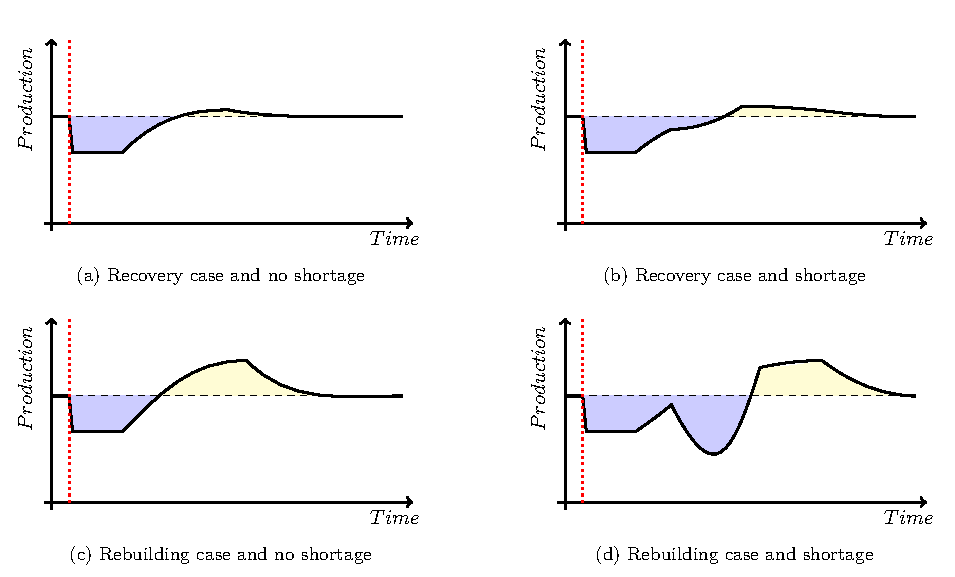
\includegraphics[width=0.9\textwidth]{imgs/ARIO-basic-responses}
  \caption[ARIO elementary responses]{ARIO elementary responses. The red dotted
    line represent a shock happening. The blue and yellow areas represent respectively the production
    losses and gains relative to a counterfactual with no shock. See a more detailed
    description in~\cref{sec:qualitative-behavior}.\label{fig:ario-responses}}
\end{figure*}

\begin{enumerate}
\item[a)] When the industry does not have to answer a reconstruction demand and
  no shortage happens (either because the shock is too small or the parameters
  are not too constraining), the industry first suffers a loss of production for the
  duration of the event and then slowly regains its production output \emph{via} the
  recovery as well as the overproduction mechanism (the actual shape of the
  curve during this recovery phase depends on whether a reconstruction demand
  affects other industries, and if not, on the functional form of the exogenous
  recovery of production capacity\footnote{In this thesis, for the recovery case, we present results
    using a linear recovery function, but the implementation allow for convex or
    concave functions, as well as custom ones. We ran simulations that we do not
    present here and found it to have only a marginal influence compared to
    other modeling choices.}). Possibly, a small overshoot to refill possible
  remaining gaps in inventories can be observed before initial equilibrium is found again.
\item[b)] If a shortage does happen, it slows down the recovery of the production
  to its initial amount, extending the recovery period. It
  may also slightly increase the overshoot in production as inventory
  gaps are increased by the longer recovery.
\item[c)] When the industry answers a reconstruction demand, but no shortage occurs,
  production rises more sharply in response to the increased scarcity created
  by the rebuilding demand. Production also continues to increase for a longer time, as
  long as total demand is not met. Once production meets total demand, it starts
  decreasing toward the initial level as the remaining reconstruction demand and
  inventory gaps are answered.
\item[d)] When a shortage happens while the industry has to answer a rebuilding
  demand, production reduces to match the constraint from its inventories.
  As long as total demand remains higher than production for the input(s)
  responsible for the shortage, the inventory gap continues to increase,
  and thus, the production to decrease. This stops when production becomes low enough
  and received orders high enough, such that the inventory gap starts decreasing
  (the inflexion point of the drop in production).
  Production then increases back as in the last phase of c), but more sharply, here,
  due to a higher remaining demand from orders to refill inventories and reconstruction.
\end{enumerate}

As stated previously, actual responses are of course more complex, as
interrelations between industries create feedback. As such, shortages can occur
at earlier or later steps, possibly at multiple times (for instance due to
different inputs), and can also overlap.

\subsection{Hypotheses, limitation, and specifics}
\label{sec:hypotheses-lim-spec}

Building hybrid or agent-based models such as the ARIO model requires a trade-off between
the simplicity of the mechanisms described and the amount of parameters
to calibrate, and therefore the transparency of modeled impacts. Considering
both the conceptual model or its implementation, several hypotheses
are made, and several limitations exist.

\subsubsection{Hypotheses}
\label{sec:hypotheses}

\begin{itemize}
\item The production is Leontief-based: no substitution is possible between different
  inputs.
\item Conversely, goods produced in the same sector but in different locations are perfect
  substitutes.
\item Industries can always hire (for overproduction), there is no limit to the
  amount of available workers.
\item Industries as well as households can always buy final products (they are
  not limited by a budget).
\item Productive capital has a constant return to scale.
\end{itemize}

\subsubsection{Limitations}
\label{sec:limitations}

There are notable limitations associated with the mechanisms represented or not
in our version of the ARIO model. A significant one comes with the absence of
prices in the model, leading economic agents to make decision based on
mechanistic rules rather than through the more realistic optimization of a
balance between profit and expenses. The implementation of such dynamics would
however introduce a substantial layer of complexity to the model and requires
careful consideration.

In parallel, the overproduction mechanism in the model is not associated with
extra costs and is only constrained by a maximum level and an inertia of
deployment. This is an overoptimistic scenario in which all industries in the
world have idle capacity only constrained by a lack of demand. We can assume
that including such price and costs dynamics would change the distribution of
impacts across regions, as production becomes more or less profitable depending
on associated hypotheses. We can also safely assume that putting a constraint on
overproduction would overall increase the indirect impacts
(see~\Cref{ch_sensitivity}).

Additionally, our consideration of final demand could be enhanced: it currently
remains fixed at each step while shifts in consumption behavior following a
natural disaster have been observed \parencite{kennett-hensel-2012-limin-consum,
  alatrista-salas-2021-impac-natur}. We do consider a ``shift'' in demand
\emph{via} the reconstruction demand, but this currently remains independent
from the households final demand, though we can assume shifts in final demand to
have similar effects as changes in the reconstruction demand.

Furthermore our implementation does not account for the role of labor (notably
the reduction in production capacity due to workers not being able to work
during the event).

\subsection{Python implementation - BoARIO}
\label{sec:implementation}

BoARIO is the python object oriented implementation we developed during this
thesis. An extensive documentation, with installation instructions, examples, as
well as a fully documented \acrfull{API} is available at
\url{https://spjuhel.github.io/BoARIO}.

The objective of this package is to offer a generic, modular, extensible and
inter-operable implementation of the ARIO model for the following reasons:
\begin{enumerate}
\item More transparent research - Indeed, although ARIO is a well used model in
  the literature on indirect economic costs, we often found it difficult to find which
  alternatives were used, with which parameters. As the model has been shown to
  be very sensitive to its parameters, this may pose an issue when interpreting
  results.
\item Ease comparison of the influence of economic data - BoARIO brings a very
  generic way to use MRIOT, making it easy to compare results with various
  sources of data.
\item Ease comparison of mechanisms - Although it does not implement all
  existing alternatives of the ARIO model, BoARIO aims at being easily extended
  with additional modules, which could simplify the evaluation of how modeling
  choices affects results.
\item Ease integration with other models - BoARIO is fairly easy to work
  with direct impact models, as its coupling with the CLIMADA modeling platform
  realised during this thesis has already shown.
\item More reproducible research - BoARIO offers a relatively simple interface
  which allows to easily reproduce simulations done in studies using the
  package. Furthermore, it is fully compatible with simulation pipeline using
  Snakemake \parencite{koester-2012-snakem-scalab}. We aim for such pipelines to
  be easily implemented, in order to make studies with BoARIO reproducible in a
  matter of a few lines of code.
\end{enumerate}

The package can be install via pip or conda using the conda-forge channel:
\begin{lstlisting}[language=bash]
  pip install boario
  # or
  conda install -c conda-forge boario
\end{lstlisting}

Furthermore the package has been submitted to the Journal of Open Source
Software (JOSS). The reviewing process is publicly available here:
\url{https://github.com/openjournals/joss-reviews/issues/6307}.

\section{Detailed description}
\label{sec:full-description-ARIO}

\subsection{Notations}
\label{sec:notations}

In this section we
provide the notations we will use throughout this thesis:

\begin{itemize}
\item We use double-barre capital letters for sets of elements (e.g., $\sectorsset$)
\item We use $|\sectorsset|$ to denote the cardinality (number of elements) of a
  set.
\item Although we will mostly avoid it, when context is sufficient, we will
  confuse indices values with what they represent (e.g., sector numbered 1 with
  1)
\item As one key hypothesis we assume that sectors produce only one
  commodity, service, or product, and we will not distinguish sectors
  and the product they produce in the notations, although we will try to favor
  $p$ over $f$ (industry) or $i$ (sector) when talking about the product.
\item Matrices, respectively vectors, will be noted using a capital,
  respectively lowercase, bold letter, while their internal elements will be
  noted with the corresponding lowercase non-bold letter.
\item We use the Hadamard product (element-wise product of two matrices), noted $A = B
  \odot C$ such that $a_{ij} = b_{ij} \cdot c_{ij} \forall i,j$.
\item We make use of generic term notation for matrices and vectors. For
  instance, $A = B \odot C$ can also be noted $A = (a_{ij}) = (b_{i,j} \cdot
  c_{i,j})$.
\item We also use element-wise division of matrices, and in order to account for
  possibly null flows we require dividing by zero to be defined. Specifically,
  if we have two matrices $A = (a_{ij})$ and $B = (b_{ij})$ of
  the same size $m \times n$, we define the ``Hadamard'' division, denoted by $A
  \oslash B = C$ where each element $c_{ij}$ of $C$ is given by:
  \[
    c_{ij} =
    \begin{cases}
      \dfrac{a_{ij}}{b_{ij}} & \text{if } b_{ij} \neq 0\\
      0 & \text{if } b_{ij} = 0
    \end{cases}
  \]
\item We will denote by $\bm{e}_{m \times n}$ the $m \times n$ matrix with all
  elements equal to $e$. For simplicity we will write, $\bm{e}_n = \bm{e}_{n
    \times 1}$ the column vector repeating $e$, $n$ times. When $e$ is not a
  scalar, we will use the bracket notation: for
  instance, $\begin{bmatrix}\bm{v}\end{bmatrix}_{1 \times q}
  = \begin{bmatrix}\bm{v} \hdots \bm{v}  \end{bmatrix}$ where $v$ is repeated $q$ times.
\item We use the Kronecker product ($\otimes$) with previously defined vectors,
  to repeat rows or columns a certain number of time (for instance
  $A \otimes \bm{1}_q$ represents matrix $A$
  where each row is repeated $q$ times):
  \[
    A \otimes \bm{1}_q =
    \begin{bmatrix}
      a_{11} & \hdots & a_{n1} \\
      \vdots & \ddots & \vdots \\
      a_{1m} & \hdots & a_{nm} \\
    \end{bmatrix}
    \otimes
    \begin{bmatrix}
      1\\
      \vdots\\
      1
    \end{bmatrix} =
    \begin{bmatrix}
      a_{11} & \hdots & a_{n1} \\
             & \vdots  & q\textrm{\scriptsize{} times} \\
      a_{11} & \hdots & a_{n1} \\
             & \vdots & \\
      a_{1m} & \hdots & a_{nm} \\
             & \vdots & q\textrm{\scriptsize{} times} \\
      a_{1m} & \hdots & a_{nm}
    \end{bmatrix}
  \]
\item As much as possible, flows from an element to another will be denoted as
  subscripts (e.g., flow of industry $f$ to industry $f^{\prime}$ is noted
  $z_{ff^{\prime}}$)
\item Conversely, superscripts will denote a particular form of a variable (e.g,
  $k_f$ the capital of $f$ and $k_f^{\textrm{Affected}}$ the subpart of capital
  of $f$ impacted).
\end{itemize}

{\renewcommand{\arraystretch}{1.3}%

  \begin{table}[H]
    \centering
    \caption{Notations table}
    \begin{tabularx}{\linewidth}{
      p{4.5cm}Xc
      }
      \textbf{Notation} & \textbf{Description} & \textbf{Dimension} \\\toprule
      $\sectorsset{} = \{ S_1, \ldots, S_n\}$ & Set of sectors indices & $|\sectorsset| = n$ \\
      $\regionsset = \{ R_1, \ldots, R_m\}$ & Set of regions indices (countries) & $|\regionsset| = m$ \\
      $\rfirmsset = \{f^R_1, \ldots,  f^R_n\}$ & Set of industries of country $R$ ($f^R_{S}$ is the industry of sector $S$ of region $R$) & $|\rfirmsset{}| = n$\\
      $\firmsset = \{\rfirmsset[R_1], \ldots, \rfirmsset[R_{m}]\}$ & Global set
                                                                     of
                                                                     industries
                                                                     (a sector
                                                                     in a
                                                                     region)
                                                                     indices. &
                                                                                $|\firmsset|
                                                                                =
                                                                                n
                                                                                \times
                                                                                m
                                                                                =
                                                                                q$\\
                                                                                % $\ioz^{RR^{\prime}}$ & Inter-regional transaction matrix & $\ioz^{RR^{\prime}} =
                                                                                % (z_{ff^{\prime}}^{RR^{\prime}})_{\substack{f
                                                                                % \in
                                                                                % \rfirmsset[R]\\f^{\prime}
                                                                                % \in \rfirmsset[R^{\prime}]\\(R,R^{\prime}) \in \regionsset}}$ \\
      $\ioz$ & Global transaction matrix (flows from $f$ to $f^{\prime}$) & $\ioz = (z_{ff^{\prime}})_{f,f^{\prime} \in \firmsset}$ \\
      % $\ioy^{RR^{\prime}}$ & Inter-regional final demand matrix & $\ioy^{RR^{\prime}} =  (y_{f}^{RR^{\prime}})_{\substack{f \in \rfirmsset\\(R,R^{\prime}) \in \regionsset}}$ \\
      $\ioy$ & Global final demand matrix (flows from $f$ to $R$) & $\ioy = (y_{fR})_{f \in \firmsset}$ \\
      % $\iov^R = \begin{bmatrix} v^{R}_{1} & \cdots & v^{R}_{n} \end{bmatrix}$ & Regional value added vector & $\iov^R =  (v_{f}^R)_{\substack{f \in \rfirmsset[R]\\R \in \regionsset}}$ \\
      $\iov$ & Global value added vector & $\iov =  (v_{f})_{f \in \firmsset}$ \\
      % $\iok^R = \begin{bmatrix} k^{R}_{1} & \cdots & k^{R}_{n} \end{bmatrix}$ & Regional capital stock vector & $\iok^R =  (k_{f}^R)_{\substack{f \in \rfirmsset[R]\\R \in \regionsset}}$ \\
      $\iok$ & Global capital stock vector & $\iok =  (k_{f})_{f \in \firmsset}$ \\
      $\iox$ & Production vector & $\iox = (x_{f})_{f \in \firmsset}$ \\
      % $\ioa^{RR^{\prime}}$ & Inter-regional technical coefficients matrix & $\ioa^{RR^{\prime}} =  (a_{f,f^{\prime}}^{RR^{\prime}})_{\substack{f \in \rfirmsset[R]\\f^{\prime} \in \rfirmsset[R^{\prime}]\\(R,R^{\prime}) \in \regionsset}}$ \\
      $\ioa$ & Global technical coefficients matrix & $\ioa =  (a_{ff^{\prime}})_{f,f^{\prime} \in \firmsset}$ \\
      % $\ioava = (a^{\textrm{va}}_{f})_{f \in \firmsset}$ & Global value added technical coefficients matrix & \\
      $\ioinv$ & Inventories/Inputs stock matrix (industry $f$'s stock of
                 product $p$) & $\ioinv = (\omega_{pf})_{\substack{f \in \firmsset\\ p \in \sectorsset}}$ \\
      $\Damage^{\textrm{Agg}}_{\textrm{Tot}}$ & Vector of per industry total capital lost
                                                from all event(s), aggregated
                                                over all types of capital (products) &
                                                                                      $\Damage^{\textrm{Agg}}_{\textrm{Tot}}
                                                                                      =
                                                                                      (\damage^{\textrm{Agg}}_{f})_{f
                                                                                      \in
                                                                                      \firmsset}$\\
      $\cdot(t)$ & Value of $\cdot$ at step $t$, where $\cdot$ can be any scalar, vector or matrix & \\
      $\psi$ & Inventories heterogeneity parameter & scalar in $[0,1]$ \\
      $\alpha^b$ & Base overproduction capacity (same for all sectors and regions) & scalar \\
      $\alpha^{\textrm{max}}$ & Maximum overproduction capacity & scalar \\
      $\tau^{\alpha}$ & Overproduction increase/decrease characteristic time &
                                                                               scalar \\
      $\bm{\tau}^{\textrm{Inv}} = \left( \tau^{\textrm{Inv}}_p \right )_{p \in \sectorsset}$ & Characteristic time of inventory restoration & vector \\
      $\tau^{E,\textrm{Rebuild}}$ & Characteristic time of rebuilding for event $E$ & scalar \\
      $\bm{s}$ & Initial/Objective inventory vector & $\bm{s} = (s_{p})_{p \in \sectorsset}$ \\
      $\bm{\kappa}$ & Capital stock to value added ratio & $\bm{\kappa} = (\kappa_{i})_{i \in \sectorsset}$ \\
      \bottomrule
    \end{tabularx}
  \end{table}
}

\subsection{Detailed model description}
\label{sec:deta-model-descr}

\subsubsection{Initial state}
\label{par:init_sh}

Initial values for intermediate demand ($\ioz(t=0)$), final consumption (or final demand)
($\ioy(t=0)$) and production ($\iox(t=0)$) are derived from MRIOTs. We also
compute initial value added ($\iov$) as the difference between production (gross
output) and intermediate demand, from which we estimate the stock of productive
capital (see~\cref{tab:capital-va-ratio} for further details). Initial
inventories ($\ioinv(t=0)$) are equal to the initial intermediate demand aggregated
by sectors (as we consider that industries of the same sectors in different region
produce the same product) which is multiplied by a chosen number $s$ of days (which can
be set on a per input basis). These initial values comply with Leontief's IO
principles, using:
\begin{itemize}
\item $\bm{i}$, a summation column vector of size $n \times m = q$ (total
  number of industries), such that $\ioz \cdot \bm{i}$ is the column vector corresponding to the
  sum of each row of $\ioz$.
\item $\bm{j}$, a summation row vector of size $n \times m = q$ (total number
  of industry), such that $\ioz \cdot \bm{j}$ is the row vector corresponding to the
  sum of each column of $\ioz$.
\item $\bm{\hat{x}}_0$, the diagonal matrix with the elements of $\iox_0$.
\end{itemize}

We have:
\begin{gather*}
  \iox_0 = \ioz \cdot \bm{i} + \ioy \cdot \bm{i}\\
  \ioa = \ioz \cdot \bm{\hat{x}}_0^{-1}\\
  % \ioava = \ioy \cdot \bm{\hat{x}}_0^{-1}
  \iov = \iox - \left ( \ioz \cdot \bm{j} \right )\\
  \iok = \bm{\kappa} \odot \iov
\end{gather*}


\notebox{
  Note that depending on the input data and the chosen temporal granularity, the
  values from the tables are divided to obtain the values by step (e.g. if the
  given MRIOT have yearly values and one step is one day, we divide by 365). Thus
  assuming no seasonality in production.
}

We also compute technology and transactions information at the sector level,
that is, regardless of the region of provenance. Let:
\[
  \bm{I^{\textrm{sum}}} =
  \underbrace{
    \begin{bmatrix}
      1 & \cdots & 0 & & 1 & \cdots & 0 \\
      \vdots & \ddots & \vdots & \cdots & \vdots & \ddots & \vdots \\
      0 & \cdots & 1 & & 0 & \cdots & 1
    \end{bmatrix}
  }_{q} n
\]

We define:
\begin{gather*}
  \ioa^{\sectorsset} = \bm{I^{\textrm{sum}}} \cdot  \ioa\\
  \ioz^{\sectorsset} = \bm{I^{\textrm{sum}}} \cdot  \ioz\\
  \ioz^{\textrm{Share}} =  \ioz \oslash \left ( \ioz^{\sectorsset} \otimes
    \bm{1}_m \right )
\end{gather*}

Hence, $\ioa^{\sectorsset}$ and $\ioz^{\sectorsset}$ are respectfully the
technical matrix and the intermediate demand matrix aggregated by
product/input, and $\ioz^{\textrm{Share}}$ represents for each firm and for each of
their input, the initial share ordered to a specific supplier relative to the
total order for this input (i.e. intermediate consumption normalized for each
input).

As stated previously, the initial inventory matrix $\ioinv$ is initialized as follows :

\begin{equation*}
  \begin{aligned}
    \ioinv(t=0) & =
                  \begin{bmatrix}\bm{s}^\intercal\end{bmatrix}_{1 \times q}
                  \otimes
                  \begin{bmatrix} \iox(0) \end{bmatrix}_{n} \odot \ioa^{\sectorsset} \\
                & = \colvec{s_1 x_1(0) a_{11} \cdots s_1 x_{q}(0) a_{1q}}{s_n x_{1}(0) a_{n1} \cdots s_n x_{q}(0) a_{nq}}
  \end{aligned}
\end{equation*}

Or more simply, using generic term notation:

\begin{center}
  $\ioinv(t=0) = \mdefentry{\omega}[0][p][\sectorsset][f][\firmsset][][]$
  with $\omega_{pf}(0) = s_p \cdot x_{f}(0) \cdot a_{pf}$
\end{center}

\tipbox{
  In plain words, $\omega_{pf}(0)$ is the exact amount of product $p$ required by industry $f$ to
  produce $x_f(0)$ (i.e. the initial equilibrium production of $f$) during $s_p$
  temporal units. Or, alternatively, that $f$ could (technically) produce during
  $s_p$ temporal units without receiving input of product $p$.
}


\subsubsection{Events, damages and production capacity reduction}
\label{par:damages_sh}

This version of the ARIO model is event-based (notably for the
purpose of multi-event simulation) and in line
with~\textcite{otto-2020-event-based}, which suggest event-based models are
better suited for evaluating impacts from extreme events.

During a simulation, the model is impacted by one or multiple events, defined by:
\begin{itemize}
\item a step of occurrence (i.e., the moment the shock happens).
\item an impact, on productive or non-productive capital, on production capacity
  directly, on final demand, or any combination of these, defined for each firms of $\firmsset$.
\item a duration (i.e. the period during which the economy fully suffers the
  impact).
\item a characteristic time of recovery ($\tau_{\textrm{Recovery}}$ or $\tau_{\textrm{Rebuild}}$).
\item a possible reconstruction demand (most often equal to the capital impacted
  (productive or non-productive)).
\end{itemize}


\paragraph{Arbitrary production capacity reduction}
\label{sec:arbitr-prod-capac}

The first type of impact we consider, are arbitrary impacts on production
capacity. Regardless of any material destruction, an event can reduce production
capacity of a set industries. As such for an event $E$, we define how it
arbitrarily affect production of industries at each step with the
\emph{arbitrary production capacity reduction}:

\[
  \bm{\Delta}^{\textrm{Arbitrary},E}(t) = \left (
    \delta^{\textrm{Arbitrary},E}_f(t) \right )_{f \in \firmsset}
\]

\paragraph{Productive capital destruction}
\label{sec:prod-capit-destr}

Most often though, production capacity are reduced \emph{via} the destruction of some
of their assets, hence we also define (independently), the \emph{reduction in productive
  capital} due to $E$ at $t$:

\[
  \iok^{\textrm{Affected},E}(t) = \left (k^{\textrm{Affected},E}_f(t) \right )_{f \in \firmsset}
\]

Just as in~\textcite{hallegatte-2013-model-role}, reduction in
production capacity from destroyed capital is simply the ratio of direct damages
over total productive capital, hence total reduction in production capacity for
event $E$ is:

\[
  \bm{\Delta}^{E}(t) = \left ( \delta^{\textrm{Arbitrary},E}_f(t) +
    \frac{k^{\textrm{Affected},E}_f(t)}{k_f} \right )_{f \in \firmsset}
\]

\paragraph{Impacts on demand}
\label{sec:impacts-demand}

Events can also impact demand, as the need to repair, replace or rebuild what was
destroyed arises. In the model we distinguish between productive and
non-productive capital, assuming destroyed households goods do not impair
production unlike industrial assets. Both these demands are defined on a
product basis (e.g., part of the demand is addressed to the Construction
sector).
Hence we define the matrices of \emph{remaining industry
  rebuilding demand} $\Damage^E(t)$ and \emph{remaining households rebuilding demand}
$\bm{\Pi}^E(t)$ as follow:

\begin{align*}
  \Damage^{E}(t) = (\damage^{E}_{pf}(t))_{\substack{f \in \firmsset\\p \in \sectorsset}} &&  \bm{\Pi}^{E}(t) = (\pi^{E}_{ph}(t))_{\substack{h \in \regionsset\\p \in \sectorsset}}
\end{align*}

Only a fraction of these remaining demands is actually
answered at time $t$, defined by the recovery/rebuilding
characteristic time (which can be set per event). The \emph{actual industry
  rebuilding demand} and the \emph{actual household rebuilding demand} are
defined as $\Damage^{E}(t) \cdot \tau^{E}_{Rebuild} $ and $\bm{\Pi}^{E}(t)
\cdot \tau^{E}_{Rebuild}$. The aggregated or total rebuilding demand
$\Damage^{\textrm{Agg}}$ is the sum of these for all events:

\label{agg_rebuilding_demand}

\[
  \Damage^{\textrm{Agg}}(t) = \sum_{\forall E} \left ( \left ( \Damage^E(t) +
    \bm{\Pi}^{E}(t) \right ) \tau^E_{\textrm{Rebuild}} \right )
\]


\subsubsection{Production}
\label{par:prod_sh}

In ARIO, production is demand-driven, which means production cannot be greater
than total demand. Another limit is the production capacity, which can change
(positively or negatively) either due to a shock (e.g. productive capital
destroyed) or due to the overproduction mechanism. Finally, production can be
constrained by the state of the inventory of inputs of an industry, the idea
being that industries aim to have enough inputs to produce at
their current production level for a given number of days. Production will
be reduced due to lack of inputs if and only if the input stock falls below the
corresponding threshold.

Hence, the production module computes the \emph{actual production} (also noted
\emph{realised production}) $\iox^a(t)$ for each industry for the
current step. To do this, it first computes the \emph{production
  capacity}, $\iox^{\textrm{Opt}}$, based on i) $\iox(0)$, ii) possible production
capacity reductions consequent to the event(s) considered ($\bm{\Delta}(t)$) and
iii) the current state of overproduction ($\bm{\alpha}(t)$). This \emph{production
  capacity} defines the absolute maximum each industry can produce at this step.

The module then computes the \emph{optimal production} (or \emph{expected
  production}) as the minimum between the \emph{total demand} (see
\cref{par:orders_sh}) and the \emph{production capacity}. Finally the module
applies possible constraints from input
inventories to compute \emph{actual production}: if the inventory for
an input is $x$\% below a certain threshold, production is reduced by $x$\% (so
that production level meets inventory constraints). Inputs required for
production are drawn from their respective inventories.

Let \(\alpha_{f}(t)\) be the overproduction factor of industry
\(f\) at $t$ and let \(\Delta_{f}(t)\) be the loss of production capacity of
industry \(f\) at $t$, production capacity of industry \(f\) at step \(t\)
before other constraints is:
\begin{equation*}
  x^{\textrm{Cap}}_{f}(t) = \alpha_{f}(t) (1 - \Delta_{f}(t)) x_{f}(t)
\end{equation*}

From production capacity, we can compute actual production $\iox^{a}(t)$, which requires the
following steps:

\paragraph{Total demand}
\label{sec:total-demand}

First we compute the total demand directed towards each industry with
Eq.~\(\text{Total demand matrix}\). Total demand is made up of orders
($\ioorders$), final demand ($\ioy$, which currently is fixed at $\ioy(0)$ for
all $t$), and aggregated reconstruction demand $\Damage^{\textrm{Agg}}$.

\paragraph{Optimal production}
\label{sec:optimal-production}

Then we compute optimal production or expected production (without considering
inventory constraints) for each industry as the minimum between production
capacity (possibly reduced by damages) and total demand, assuming an industry
will not produce more than it is asked for (Eq.~\(\text{Optimal production}\)).

\paragraph{Inventory constraints}
\label{sec:invent-constr}
We define inventory constraints \(\ioinv^{\textrm{Cons}}\) for each input, as a
share \(\psi\) of the amount of stocks required to produce \(s_p^f\) steps of
production at the \emph{optimal production} level (Eq.~\(\text{Inventory
  constraints}\)).

{ \small
  \begin{alignat*}{4}
    \bm{D}^{\textrm{Tot}}(t) &= (d_{f}^{\textrm{Tot}}(t))_{f \in \firmsset} &&=
                                                                               \ioorders(t)
                                                                               \cdot
                                                                               \irowsum{q}
                                                                               +
                                                                               \ioy(t)
                                                                               \cdot
                                                                               \irowsum{q}
                                                                               +
                                                                               \Damage^{\textrm{Agg}}(t)
    \cdot \irowsum{q} && \text{Total demand matrix} \\
                                 & && &&\\
    \iox^{\textrm{Opt}}(t) &= (x^{\textrm{Opt}}_{f}(t))_{f \in \firmsset} &&= \left ( \min \left ( d^{\textrm{Tot}}_{f}(t), x^{\textrm{Cap}}_{f}(t) \right ) \right )_{f \in \firmsset} && \text{Optimal production}\\
                                 & && &&\\
    \ioinv^{\textrm{Req}}(t) &= (\omega^{\textrm{Cons}}_{pf}(t))_{\substack{p \in \sectorsset\\f \in \firmsset}} &&=
                                                                                                                  \begin{bmatrix}
                                                                                                                    s_{11} & \cdots & s_{1q} \\
                                                                                                                    \vdots & \ddots & \vdots\\
                                                                                                                    s_{n1} & \cdots & s_{nq}
                                                                                                                  \end{bmatrix}
                                                                                                                  \odot \begin{bmatrix} \iox^{\textrm{Opt}}(t) \end{bmatrix}_{n} \odot \ioa^{\sectorsset} \cdot \psi &                                    & \\
                                                                                                                                                                                             &                                    &  & = \begin{bmatrix}
                                   s_{11} x^{\textrm{Opt}}_{1}(t) a_{11}                                                                                                                     & \cdots                             & s_{1q} x^{\textrm{Opt}}_{q}(t) a_{1q}\\
                                   \vdots                                                                                                                                                    & \ddots                             & \vdots\\
                                   s_{n1} x^{\textrm{Opt}}_{1}(t) a_{n1}                                                                                                                     & \cdots                             & s_{nq} x^{\textrm{Opt}}_{q}(t) a_{nq}
                                 \end{bmatrix}
                                     \cdot \psi                                                                                                                                              &                                    & \text{Inventory constraints}  \\
                                                                                                                                                                                             &                                    &  &  &  & \\
                                                                                                                                                                                             &                                    &  & = \left ( s_{pf} \cdot x^{\textrm{Opt}}_f(t) \cdot
                                     a_{pf} \cdot \psi \right )_{\substack{p \in \sectorsset\\f \in \firmsset}} \\
                                                                                                                                                                                             &                                    &  &  &  & \\
    \iox^{a}(t)                                                                                                                                                                              & = (x^{a}_{f}(t))_{f \in \firmsset} &  & = \left \{ \begin{aligned}
                                                                                                                                                                                             & x^{\textrm{Opt}}_{f}(t)            & \text{if } \forall p, \omega_{pf}(t) \geq \omega^{\textrm{Cons}}_{pf}(t)\\
                                                                                                                                                                                             & x^{\textrm{Opt}}_{f}(t) \cdot \min_{p \in \sectorsset} \left (
        \frac{\omega_{pf}(t)}{\omega^{\textrm{Req}}_{pf}(t)} \right )                                                                                                                        & \text{if }
                                                                       \exists p, \omega_{pf}(t) < \omega^{\textrm{Req}}_{pf}(t)
    \end{aligned} \right. \quad                                                                                                                                                              &                                    & \text{Actual production at $t$}
  \end{alignat*}
}%

\notebox{
  Note that several inventory constraints alternative definition can be thought of,
  for example by using $\iox^{a}(t-1)$, $\iox^{\textrm{Cap}}(t)$ or $\iox^{\textrm{Opt}}(t-1)$ in
  place of $\iox^{Opt}(t)$. In~\textcite{hallegatte-2013-model-role},
  the author states that he uses $\iox^{a}(t-1)$ in the model description, while
  the code we obtain clearly uses $\iox^{\textrm{Opt}}(t)$. We also found this
  alternative to be less prone to \emph{whip effects}, where production and
  demand oscillate importantly from one step to another. We suggest greater
  consideration to this aspect of the model should be studied in the future.
}

If the inventory of product \(p \in \sectorsset\) of an industry \(f\) is lower
than its required level, then \(f\)’s production is reduced. An inventory
shortage of \(x\) \% (w.r.t. its constraint) leads to a \(x\) \% reduction of
production. When an industry enters such a state, where it ``choose'' to
reduce its production level in view of its inventories being insufficient in the
long run, we say the industry enters a ``\emph{shortage regime}''.

\subsubsection{Distribution}
\label{sec:distribution}

The distribution module distributes the \emph{actual production} of each industry
to the different demands.

\paragraph{Rationing scheme}
\label{sec:rationing-scheme}

Distribution follows a proportional rationing scheme: \emph{intermediate orders} $\ioorders(t)$, \emph{final demand}
$\ioy(t)$, \emph{aggregated rebuilding demand} $\Damage^{\textrm{Agg}}(t)$ each
receive their relative share of the \emph{total demand} of the \emph{actual
  production}.

Hence, if \(d_f^{\textrm{Tot}}(t) = x_f(t)\), each client receive their full order. While if \(d_f^{\textrm{Tot}}(t) > x_f(t)\),
each client receive only part of it, let:
\begin{itemize}
\item $o_{ff^{\prime}}(t)$, the amount ordered by $f^{\prime}$ to $f$
\item $y_{fh}$, the amount of final demand from households in region $h$ addressed to $f$
\item $\damage^{E}_{ff^{\prime}}(t)$, the amount of damage on the capital of industry
  $f^{\prime}$ rebuilt \emph{via} industry $f$ for event $E$.
\item $\damage^{E}_{fh}(t)$, the amount of damage on the capital of
  households in region $h$ rebuilt \emph{via} industry $f$ for event $E$.
\end{itemize}

We can define:
\begin{alignat*}{4}
  &\ioorders^{\textrm{Received}}(t) &&= \left ( \frac{o_{ff^{\prime}}(t)}{d^{\textrm{Tot}}_f(t)} \cdot x^a_f(t) \right )_{f,f^{\prime}\in \firmsset}\\
  &\ioy^{\textrm{Received}}(t) &&= \left (
                                  \frac{y_{fh}}{d^{\textrm{Tot}}_f(t)}\cdot
                                  x^a_f(t) \right )_{\substack{f\in \firmsset\\h
  \in \regionsset}}\\
  &\Damage^{\textrm{Repaired}}(t) &&= \left ( \frac{\damage^{E}_{ff^{\prime}}(t)
                                     }{d^{\textrm{Tot}}_f(t)} \cdot x^a_f(t)
                                     \right )_{\substack{\forall E\\f,f^{\prime}\in \firmsset}}\\
  &\bm{\Pi}^{\textrm{Repaired}}(t) &&= \left ( \frac{\pi^{E}_{fh}
                                      }{d^{\textrm{Tot}}_f(t)} \cdot x^a_f(t)
                                      \right )_{\substack{\forall E\\f\in \firmsset\\h\in \regionsset}}\\
\end{alignat*}


\notebox{
 The rationing scheme plays a key role in the propagation of indirect impacts,
 and other scheme should also be considered, for instance ones that prioritize
 intermediate demand over final demand, or domestic demand over exports. Such
 scheme, where a priority is define, require multiple rounds of distribution
 which induces more computation. As the proportional scheme is the most used
 in the existing literature, we only developed this one, but we consider adding
 other scheme in further development of the model.
}


\paragraph{Inventory resupply}
\label{sec:inventory-resupply}


From these values the model can compute the new state of the inventory of each
firm:

\begin{alignat*}{4}
  &\ioinv(t+1) &&= \ioinv(t) + \underbrace{ \bm{I}^{\textrm{sum}} \cdot
                  \ioorders^{\textrm{Received}}(t) }_{\text{orders received
                  aggregated by products}} - \underbrace{\begin{bmatrix} \iox^{\textrm{a}}(t) \end{bmatrix}_{n} \odot \ioa^{\sectorsset}}_{\text{inputs used during production}}\\
\end{alignat*}

\paragraph{Rebuilding}
\label{sec:rebuilding}


For each event, for each impacted industry or household, the remaining damages
to rebuild at $t$ are simply the remaining damages at $t-1$ minus what was repaired:

\begin{align*}
  \Damage^{E}(t+1) &= (\damage^{E}_{pf}(t) - \damage^{\textrm{Repaired},E}_{pf}(t) )_{\substack{f \in \firmsset\\p \in \sectorsset}}\\
  \bm{\Pi}^{E}(t+1) &= (\pi^{E}_{ph}(t) - \pi^{\textrm{Repaired},E}_{ph}(t))_{\substack{h \in \regionsset\\p \in \sectorsset}}\\
\end{align*}

\subsubsection{Orders}
\label{par:orders_sh}

The orders module computes the demands made by the different agents to be
answered at the next step:
\begin{itemize}
\item The intermediate demand, from industries aiming at refilling their
  inventories of inputs.
\item The final demand \footnote{Although we use the term households for the
    sake of simplicity, final demand actually also comprehend the demand from government
    expenditures and private sector final demand such as capital formation.}, which in the current
  version of the model stays fixed throughout the simulation.
\item The possible rebuilding demand remaining.
\end{itemize}

\notebox{
 ~\Textcite{hallegatte-2008-adapt-region} implemented a
macro-effect on the final demand which is not included in our version. Although
the author shows this mechanism has limited impact on results \emph{via} a sensitivity
analysis, we aim at including a similar mechanism in later developments.
}

\paragraph{Intermediate orders}
\label{sec:intermediate-orders}

Intermediate orders are decided based on inventories and consists of two parts:
the amount of inputs used to produce during the current step, and a fraction
$1 / \tau^{\textrm{Inv}}_{p}$ of the gap between current inventories and
objective for input $p$.
Inventory objectives are defined relative to \emph{optimal production}:

An industry $f$ seeks to maintain a level of input $p$ so that it can produce
$x^{\textrm{Opt}}_f$  during $s_p$ steps. As such, if $x^{\textrm{Opt}}_f(t)$ is
higher (or lower) than $x_f(0)$, the actual amount of $p$ required will be
higher (respectively lower).

\begin{alignat*}{4}
  &\ioinv^{*}(t) &&= (\omega_{pf}^{*}(t))_{\substack{p \in \sectorsset\\f \in \firmsset}} \quad = \quad s_{pf} \cdot \begin{bmatrix} \iox^{\textrm{Opt}}(t) \end{bmatrix}_{n} \odot  \ioa^\sectorsset && \quad && \text{Inventory goals} \\
  &\ioinv^{\textrm{Gap}}(t) &&= (\omega_{pf}^{\textrm{Gap}}(t))_{\substack{p \in \sectorsset\\f \in \firmsset}} \quad = \quad \left ( \ioinv^{*} - \ioinv(t) \right )_{\geq 0} && \quad && \text{Inventory gaps}\\
\end{alignat*}

Where $(\bm{A} - \bm{B})_{\geq 0}$ denotes the resulting matrix of $A -
B$ where negative values are replaced by 0 (If inventories are higher than the
objective, then there is no need to refill them).

\begin{alignat*}{4}
  & \ioorders^{\sectorsset}(t) &  & = \begin{bmatrix}
    \iox^a(t) \end{bmatrix}_{n} \odot  \ioa^{\sectorsset} + \begin{bmatrix} 1 / \tau^{\textrm{Inv}}_1 \hdots 1 / \tau^{\textrm{Inv}}_n  \end{bmatrix} \odot \ioinv^{\textrm{Gap}}(t) &  & \quad &  & \text{Intermediate demand total orders}\\
 & \ioorders(t)               &  & = \left ( \ioorders^{\sectorsset}(t) \otimes \bm{1}_{m} \right ) \odot  {\textcolor{OliveGreen}{\ioz^{\textrm{*}}}} &  & \quad &  & \text{Intermediate demand orders}
\end{alignat*}

We actually implement two different ways orders are made, which differ here in
the definition of ${\textcolor{OliveGreen}{\ioz^{\textrm{*}}}}$:

\begin{enumerate}
\item The model uses the initial transaction shares: $\ioz^{\textrm{*}}(t) =
  \ioz^{\textrm{Share}}$, just as in
 ~\textcite{hallegatte-2013-model-role}. In this case there is no
  substitution possible among supplier. As a reminder:
  \[
  \begin{split}
    \ioz^{\textrm{Share}} =  \ioz \oslash \left ( \left (
    \bm{I^{\textrm{sum}}} \cdot  \ioz \right ) \otimes
    \bm{1}_{m}
    \right )
  \end{split}
\]
\item The model uses the initial transaction share, but now weighted by the
  current production level of suppliers, relative to their initial production. This
  is done by replacing both occurrences of $\ioz$ in the previous equation by
  the following:
  \[
    \begin{split}
      \ioz \odot
      \begin{bmatrix}
        \frac{x_{1}(t)}{x_{1}(0)} & \cdots & \frac{x_{p}(t)}{x_{p}(0)}\\
        \vdots & \ddots & \vdots \\
        \frac{x_{1}(t)}{x_{1}(0)} & \cdots & \frac{x_{p}(t)}{x_{p}(0)}
      \end{bmatrix}
    \end{split}
  \]
  Which corresponds to the variant defined in~\textcite{guan-2020-global-suppl}.
\end{enumerate}

\subsubsection{Overproduction}
\label{sec:overprod_sh}

The overproduction module describes how industries temporarily increase their
production when they cannot meet demand.
Overproduction increases or decreases following a base value
$\alpha^{\textrm{b}}$, a maximum value $\alpha^{\textrm{max}}$, a scarcity
index $\zeta(t)$ (unmet demand over total demand) and a characteristic time $\tau_{\alpha}$:

\begin{alignat*}{3}
  & \zeta(t) &&= \frac{d_{f}^{\textrm{Tot}}(t) - x^{a}_f(t)}{d_{f}^{\textrm{Tot}}(t)}\\
  & \alpha_f(t+1) &&= \begin{cases}
    \alpha_f(t) + (\alpha^{\textrm{max}} - \alpha_f(t)) \cdot \zeta(t) \cdot \frac{1}{\tau^{\alpha}} & \text{if } \zeta(t) > 0\\
    \alpha_f(t) +  (\alpha^{\textrm{b}}  - \alpha_f(t)) \cdot \frac{1}{\tau^{\alpha}}                & \text{if } \zeta(t) \leq 0\\
  \end{cases}
\end{alignat*}

\subsection{Parameters}
\label{sec:parameters}

\subsubsection{Capital to value added ratio}
\label{sec:capital-to-va}

The ARIO model requires an estimation of the productive capital stock of
each industry $k_f$. Although strictly speaking, this is not a model parameter,
it does play a key role in the modeling process. In~\textcite{hallegatte-2008-adapt-region}, the
author uses a fixed productive capital to value added ratio $\kappa$ of 4 (i.e., $\forall
f \in \firmsset, k_f = 4 \times v_f$). In
\textcite{hallegatte-2013-model-role}, the author assesses per sector
ratios from USA-scale data obtained from the Bureau of Economic Analysis (see
\Cref{tab:capital-va-ratio}).

\begin{table}[h]
  \centering
  \begin{tabular}{@{}ll@{}}
    \toprule
    \textbf{Sector}                         & \textbf{Ratio Capital to VA} \\ \midrule
    Agriculture, forestry, etc.             & 2.9                          \\
    Mining and extraction                   & 5.1                          \\
    Utilities                               & 4.3                          \\
    Construction                            & 0.4                          \\
    Manufacturing                           & 1.4                          \\
    Wholesale trade                         & 0.6                          \\
    Retail trade                            & 1.1                          \\
    Transportation and warehousing          & 2.7                          \\
    Information                             & 2.4                          \\
    Finance, insurance, real estate, etc.   & 6.9                          \\
    Professional and business services      & 0.5                          \\
    Educational services, health care, etc. & 1.1                          \\
    Arts, recreation, accommodation, etc.   & 1.2                          \\
    Other services, except government       & 1.2                          \\
    Government                              & 4.9 \\
    \bottomrule
  \end{tabular}%
  \caption{Productive capital to value added ratio in \textcite{hallegatte-2013-model-role}}
  \label{tab:capital-va-ratio}
\end{table}

Our version of the model offers three possibilities to define the vector of
capital stock per industry $\iok$:
\begin{itemize}
\item By default a fixed ratio of 4 is set: $\iok = 4 \cdot \iov$
\item Modelers can input a vector $\bm{\kappa}$ which define the ratio on a per
  sector basis (then $\iok = \bm{\kappa} \odot \iov$)
\item Modelers can also directly input a vector of productive capital per industry $\iok$
\end{itemize}

\tipbox{
  The STAN Industrial Analysis \textcite{horvat-2020-oecd-stan} provides
  estimates of capital stock per sector and region, for OECD countries and ISIC
  REV.4 sector typology.
}

\subsubsection{Overproduction parameters}
\label{sec:overprod-params}

As presented in~\cref{sec:overprod_sh}, overproduction in ARIO is
governed by three parameters:
\begin{itemize}
\item $\alpha^{b}$ the base overproduction factor, which should \emph{a priori}
  not differ from 1, but may be relevant in very specific case studies. For
  instance, it may be helpful to model production capacity that can be almost
  instantly increased post disaster (e.g., through disaster response planning).
\item $\alpha^{\textrm{max}}$, the maximum overproduction factor.
\item $\tau^{\alpha}$, the overproduction characteristic time (or pace), which
  represents the approximate number of days until maximum overproduction is
  reached.
\end{itemize}

These parameters are introduced in the first version of the model in
\textcite{hallegatte-2008-adapt-region}. To our knowledge the value
of $\alpha^{b}$ is always assumed to be 1 in the literature. For
$\alpha^{\textrm{max}}$, we found values ranging from the original 1.2 in
\textcite{hallegatte-2008-adapt-region} to 1.5. For $\tau^{\alpha}$,
values range from three months to a year.

\subsubsection{Heterogeneity parameter $\psi$}
\label{sec:parameter-psi}

As we presented in~\cref{sec:invent-constr}, $\psi$ governs how
industries consider the state of their inventory of inputs sufficient relative
to their current level of production. When it is close to 1, shortages and
bottlenecks are more likely to appear, or to appear sooner. In that sense,
inventories allow ARIO to be more flexible than pure IO models, but also create
the possibility of a drop in production output due to shortages.

\notebox{
As stated in~\textcite{hallegatte-2013-model-role}, if we distinguish
between industry level (branches) and firms that compose them,
$\psi$ can also be thought of as the degree of heterogeneity and possible
substitution between firms belonging to an industry:
\begin{itemize}
\item If $\psi$ is close to 0, an inventory reduction in an industry is
  homogeneously distributed among its firms: inventory reduction impacts
  industry production only if it is large enough to affect a sufficiently
  large part of the firms.
\item If $\psi$ is close to 1, an inventory reduction in an industry is
  concentrated in a few firms and forces them to stop producing which
  directly impact production on the industry level.
\end{itemize}
}

\Textcite{koks-2014-integ-direc, hallegatte-2013-model-role} highlighted the high sensitivity of the ARIO model to this
parameter. In~\textcite{hallegatte-2013-model-role}, with a value
lower of equal to 0.7, no forward propagation happens (i.e., no shortages) while
a value of 1 drastically increases the indirect losses.
\Textcite{koks-2014-integ-direc} further show how the
sensitivity itself depends on the intensity of the shock in input. They found
the value of $\psi$ to have the largest influence on the results
for 1/1000 floods (63\% of the variance) and 1/10000 floods (44\% of the
variance) and comparatively less influence for 1/100 floods (35\% of the
variance).

\subsubsection{Characteristic time of rebuilding}
\label{sec:recovery-param}

Reconstruction of destroyed assets is partially endogenous in ARIO and depends
on a characteristic time $\tau^{\textrm{Rebuild}}$ (see~\cref{sec:impacts-demand}). This parameters expressed as
a number of steps, sets the amount of the remaining destroyed assets the model
tries\footnote{Due to the rationing scheme, part of the rebuilding demand may
  not be answered.} to rebuild at each step. This parameters is not present in
ARIO's seminal paper \parencite{hallegatte-2008-adapt-region} as
in this version, intermediate demand is prioritized over reconstruction demand,
which gets only what is left once intermediate demand is satisfied. It is first
added in~\textcite{ranger-2010-asses-poten} with a value of three
months. Although not precisely stated in
\textcite{hallegatte-2013-model-role}, diving into the code shows a
value of 4 years which is used in several following papers
\parencite{zhang-2018-analy-econom, koks-2014-integ-direc} with the exception of
\textcite{avelino-2019-chall-estim} who uses 5 years. Other studies
either do not use this parameters (for instance because they use entirely
exogenous rebuilding/recovery path) or do not precise its value.
In~\textcite{koks-2019-macroec-impac}, a global scope study on
the indirect impact of floods in Europe, authors define multiple possible
recovery curves (linear, convex, S-shaped).
Each curve sets the value of parameter matching $\tau^{\textrm{Rebuild}}$ in
function of the intensity of the impacting flood. This could prove a better
alternative, as reconstruction time is deeply tied to the magnitude of a
disaster. As such, future studies should have a greater focus into this aspect
of the model.

As we show in~\Cref{ch_sensitivity}, the ARIO model can be very
sensitive to the value of this parameter. Indeed, when the reconstruction demand
per step is greater, so is the rationing of intermediate demand, which increase
the possibility of an input shortage, further leading to greater indirect
losses.

\notebox{
  Our implementation of ARIO allows to choose a specific
  $\tau^{\textrm{Rebuild}}$ per event (as well a global one), to account how
  different events take more or less time to rebuild from.
}

\subsubsection{Inventory size and resupply characteristic time}
\label{sec:inventories-params}

Inventories dynamics are governed by two parameters: $\bm{s}$, which acts both
as initial size and objective of inventories for each input, expressed in a
number of step, and $\bm{\tau}^{\textrm{Inv}}$, the characteristic time for resupply,
that is, industries aim to fill the gap between their current inventories and
their goal in approximately that time (see~\cref{sec:inventory-resupply}).

\paragraph{Inventory size}
\label{sec:inventory-size}

It is important to note here that inventory size does not necessarily represent
a physical amount of inputs (as inputs from some sectors are not material or
cannot be stocked), but rather the amount of time an industry can produce
without receiving new inputs from a given sector. Hence, inventory sizes are
defined by input, or at least by category of inputs. For instance,
\textcite{hallegatte-2013-model-role}, or
\textcite{okuyama-2004-model-spatial}, consider three types of
inventory managements for inputs: anticipatory (90 days), responsive (60 days)
and just in time (3 days). \Textcite{hallegatte-2013-model-role}
also evaluates the model sensitivity to this parameter (for anticipatory
management only), using 30, 75, 120 and 180 days. He finds the economy
collapses for $\bm{s}=30$, and that no forward impacts happen when $\bm{s} \geq
120$. As such, he shows the existence of a ``threshold in the amount of losses
an economy can cope with in the absence of external support'' and that small
inventories increase vulnerability to shocks.

Although the majority of studies using ARIO with inventories sets inventories
size similar to~\textcite{hallegatte-2013-model-role}, this parameter
is rarely discussed in depth in the literature, and often omitted
\parencite{zhang-2021-analy-impac, zhang-2017-asses-rippl, wang-2020-econom-footp, huang-2022-estim-poten}. A value of 60 days is found in~\textcite{avelino-2019-chall-estim}
\Textcite{inoue-2018-firm-simul} who use an \acrshort{ABM}
based on ARIO, calibrate inventory size using the case study of the Great East
Japan Earthquake and japan indices on industrial production, and find a value of
9 days (which we suppose is common to all agents). \Textcite{colon-2020-fragm-produc, colon-2019-trans-suppl}, build this parameters based on a survey
and use 88 different values (which average to 4.5 weeks).

\notebox{
  In the multi-regional case considerations on setting inventories size on a per
  industry (instead of sector) basis could be an improvement. Although it would be much more
  data-intensive, as it would account not only for differences in sectors but
  also in regions.
}

\paragraph{Resupply time}
\label{sec:resupply-time-param}

In~\textcite{hallegatte-2013-model-role} parameter
$\bm{\tau}^{\textrm{Inv}}$ is set to 30 days (presumably for ``anticipatory''
management), while the value for ``responsive'' and ``just in time''
is not explicit. A sensitivity analysis is also made using 7, 14, 60 and 90
days which find similar results to the analysis made on $\bm{s}$. This
parameters is also rarely discussed in the rest of the literature.
\Textcite{inoue-2018-firm-simul} use a value of 6, and other study presumably
use the value of 30 days from~\textcite{hallegatte-2013-model-role}.
\Textcite{guan-2020-global-suppl} do not explicit
the value in the study, but their open-source code uses a value of 6 weeks.

{\renewcommand{\arraystretch}{1.0}%
\begin{sidewaystable}[]
  \centering
  \resizebox{\textwidth}{!}{%
    \begin{tabular}{@{}llllllll@{}}
      \toprule
      \textbf{Articles}                                             & $\bm{\alpha^{b}}$ & $\bm{\alpha^{\textrm{max}}}$                                                                                               & $\bm{\tau^{\alpha}}$                                                                                       & $\bm{\tau^{\textrm{inv}}}$ & $\bm{s}$ (Inventory duration)                                                            & $\bm{\tau^{\textrm{Rebuild}}}$                                                 & $\bm{\psi}$ \\ \midrule
      \cite{hallegatte-2008-adapt-region}           & 1.0               & 1.0 ; 1.2 ; 1.5                                                                                                            & 3 and 6 months                                                                                             & -                          & -                                                                                        & -                                                                              & - \\[5pt] \midrule[.03em]
      \cite{ranger-2010-asses-poten}                & 1.0               & \begin{tabular}[c]{@{}l@{}}1.20\\from \cite{hallegatte-2008-adapt-region}\end{tabular}                     & \begin{tabular}[c]{@{}l@{}}6 months\\from \cite{hallegatte-2008-adapt-region}\end{tabular}  & -                          & -                                                                                        & 3 months                                                                       & - \\[5pt] \midrule[.03em]
      \cite{henriet-2012-firm-networ}              & -                 & -                                                                                                                          & -                                                                                                          & -                          & 2 to 10 days                                                                             & -                                                                              & - \\[5pt] \midrule[.03em]
      \cite{wu-2011-region-indir}   & 1.0               & 1.25                                                                                                                       & \begin{tabular}[c]{@{}l@{}}6 months\\from \cite{hallegatte-2008-adapt-region}\end{tabular}              & -                          & -                                                                                        & -                                                                              & - \\[5pt] \midrule[.03em]
      \cite{hallegatte-2013-model-role}              & 1.0               & 1.25                                                                                                                       & 1 year                                                                                                     & 7; 14; 30; 60; 90 days     & 30 ; 75 ; 90 ; 120 ; 180 days                                                            & \begin{tabular}[c]{@{}l@{}}Not explicit,\\ 4 years in source code\end{tabular} & 0.8                                                                                 \\[5pt] \midrule[.03em]
      \cite{koks-2014-integ-direc}              & 1.0               & \begin{tabular}[c]{@{}l@{}}1.25\\ from \cite{hallegatte-2013-model-role}\\ and SA on 1-3 range\end{tabular} & 6 months, 1 year, 2 years                                                                                  & Probably 30 days           & \begin{tabular}[c]{@{}l@{}}By category \\ 3 ; 60 ; 90 days\end{tabular}                  & -                                                                              & \begin{tabular}[c]{@{}l@{}}0.8 \cite{hallegatte-2013-model-role}\\ and SA on 0-1 range\end{tabular} \\[5pt] \midrule[.03em]
      \cite{zhang-2017-asses-rippl}                & 1.0               & 1 ; 1.2 ; 1.5                                                                                                              & 3-6 months                                                                                                 & -                          & -                                                                                        & -                                                                              & - \\[5pt] \midrule[.03em]
      \cite{zhang-2018-analy-econom}                & 1.0               & 1.25                                                                                                                       & 1 years                                                                                                    & 30 days                    & 90 days                                                                                  & 4 ans                                                                          & 0.8                                                                                 \\[5pt] \midrule[.03em]
      \cite{wang-2018-quant-spatial}                 & 1.0               & 1.1 to 1.5                                                                                                                 & 3m - 6m                                                                                                    & -                          & -                                                                                        & -                                                                              & - \\[5pt] \midrule[.03em]
      \cite{inoue-2019-firm-level}                 & -                 & -                                                                                                                          & -                                                                                                          & 6 days                     & 9 days from calibration                                                                  & -                                                                              & - \\[5pt] \midrule[.03em]
      \cite{colon-2019-trans-suppl}                     & 1.0               & 1                                                                                                                          & -                                                                                                          & -                          & \begin{tabular}[c]{@{}l@{}}Built from survey: 88 values\\ 4.5 weeks average\end{tabular} & -                                                                              & - \\[5pt] \midrule[.03em]
      \cite{avelino-2019-chall-estim}                      & 1.0               & 1.0                                                                                                                        & -                                                                                                          & -                          & 60 days                                                                                  & 5 years                                                                        & 1.0                                                                                 \\[5pt] \midrule[.03em]
          \cite{shughrue-2020-global-spread}        & 1                 & \begin{tabular}[c]{@{}l@{}}1.2\\from \cite{hallegatte-2008-adapt-region}\end{tabular}                      & \begin{tabular}[c]{@{}l@{}}6 months\\from \cite{hallegatte-2008-adapt-region}\end{tabular} & -                          & -                                                                                        & -                                                                              & - \\[5pt] \midrule[.03em]
          \cite{guan-2020-global-suppl} & 1.0               & \begin{tabular}[c]{@{}l@{}}1.25\\from \cite{hallegatte-2013-model-role}\end{tabular}                        & \begin{tabular}[c]{@{}l@{}}1 years\\from \cite{hallegatte-2013-model-role}\end{tabular}     & -                          & 6 week                                                                                   & -                                                                              & - \\[5pt] \midrule[.03em]
      \cite{mendoza-tinoco-2020-flood-footp-asses}                  & -                 & -                                                                                                                          & -                                                                                                          & -                          & -                                                                                        & -                                                                              & - \\[5pt] \midrule[.03em]
          \cite{huang-2020-asses-econom}                            & 1                 & 1.23                                                                                                                       & \begin{tabular}[c]{@{}l@{}}6 months\\from \cite{hallegatte-2008-adapt-region}\end{tabular} & -                          & -                                                                                        & -                                                                              & - \\[5pt] \midrule[.03em]
      \cite{wang-2020-econom-footp}                        & -                 & -                                                                                                                          & -                                                                                                          & -                          & -                                                                                        & -                                                                              & - \\[5pt] \midrule[.03em]
      \cite{colon-2020-fragm-produc}               & 1.0               & 1                                                                                                                          & -                                                                                                          & -                          & \begin{tabular}[c]{@{}l@{}}Built from survey: 88 values\\ 4.5 weeks average\end{tabular} & -                                                                              & - \\[5pt] \midrule[.03em]
      \cite{inoue-2021-propag-inter}                                & -                 & -                                                                                                                          & -                                                                                                          & 6 days                     & 10 days from \cite{inoue-2019-firm-level}                               & -                                                                              & - \\
      \bottomrule
    \end{tabular}%
  }
  \caption{ARIO parameters values throughout the literature. The absence of a
    value either indicates that the parameter did not make sense in the study,
    or that no value could be found.}
  \label{tab:parameters-lit}
\end{sidewaystable}
}
%%% Local Variables:
%%% mode: latex
%%% TeX-master: "../main"
%%% End:


\onlyinsubfile{
{\printglossary[type=\acronymtype,title=Acronyms]}
\printbibliography
}

\end{document}
%%% Local Variables:
%%% mode: LaTeX
%%% TeX-master: t
%%% TeX-engine: xetex
%%% TeX-output-dir: "./model-standalone"
%%% LaTeX-biblatex-use-Biber: t
%%% End:
